\documentclass[tikz,border=8pt]{standalone}
\usepackage[T1]{fontenc}
\usepackage{lmodern}
\usepackage{xcolor}
\usetikzlibrary{arrows.meta,positioning,fit,calc,backgrounds}
\pgfdeclarelayer{background}
\pgfsetlayers{background,main}

\definecolor{ink}{HTML}{334155}
\definecolor{line}{HTML}{64748B}
\definecolor{stagefill}{HTML}{F8FAFC}
\definecolor{queryfill}{HTML}{FFF4CC}
\definecolor{agentfill}{HTML}{F6B44B}
\definecolor{toolfill}{HTML}{DCEAF8}
\definecolor{knowfill}{HTML}{DFF3E8}
\definecolor{verifyfill}{HTML}{EDE9FE}
\definecolor{evalfill}{HTML}{FDECEC}
\definecolor{tracefill}{HTML}{F1F5F9}

\tikzset{
  font=\sffamily,
  layer/.style={
    draw=line,
    line width=0.65pt,
    fill=stagefill,
    inner xsep=5mm,
    inner ysep=7mm
  },
  layer title/.style={
    font=\sffamily\bfseries\large,
    text=black,
    fill=stagefill,
    inner xsep=2mm,
    inner ysep=0.8mm
  },
  box/.style={
    draw=line,
    line width=0.65pt,
    align=center,
    minimum height=13mm,
    text width=34mm,
    inner sep=3pt
  },
  widebox/.style={
    box,
    text width=42mm
  },
  smallbox/.style={
    box,
    minimum height=10mm,
    text width=27mm,
    font=\sffamily\footnotesize
  },
  query/.style={box, fill=queryfill},
  agent/.style={box, fill=agentfill},
  tool/.style={smallbox, fill=toolfill},
  knowledge/.style={widebox, fill=knowfill},
  verifier/.style={box, fill=verifyfill},
  eval/.style={box, fill=evalfill},
  trace/.style={box, fill=tracefill},
  arrow/.style={
    -{Latex[length=2.4mm]},
    draw=ink,
    line width=0.75pt
  },
  feedback/.style={
    -{Latex[length=2.4mm]},
    draw=ink,
    dashed,
    line width=0.75pt,
    rounded corners=2pt
  },
  observe/.style={
    -{Latex[length=2.1mm]},
    draw=ink,
    dotted,
    line width=0.75pt,
    rounded corners=2pt
  },
  flowlabel/.style={
    font=\sffamily\scriptsize,
    text=ink,
    fill=white,
    inner sep=1.2pt
  },
  side label/.style={
    rotate=90,
    font=\sffamily\Large,
    text=ink,
    align=center
  },
  side rule/.style={
    draw=ink,
    line width=0.7pt
  }
}

\begin{document}
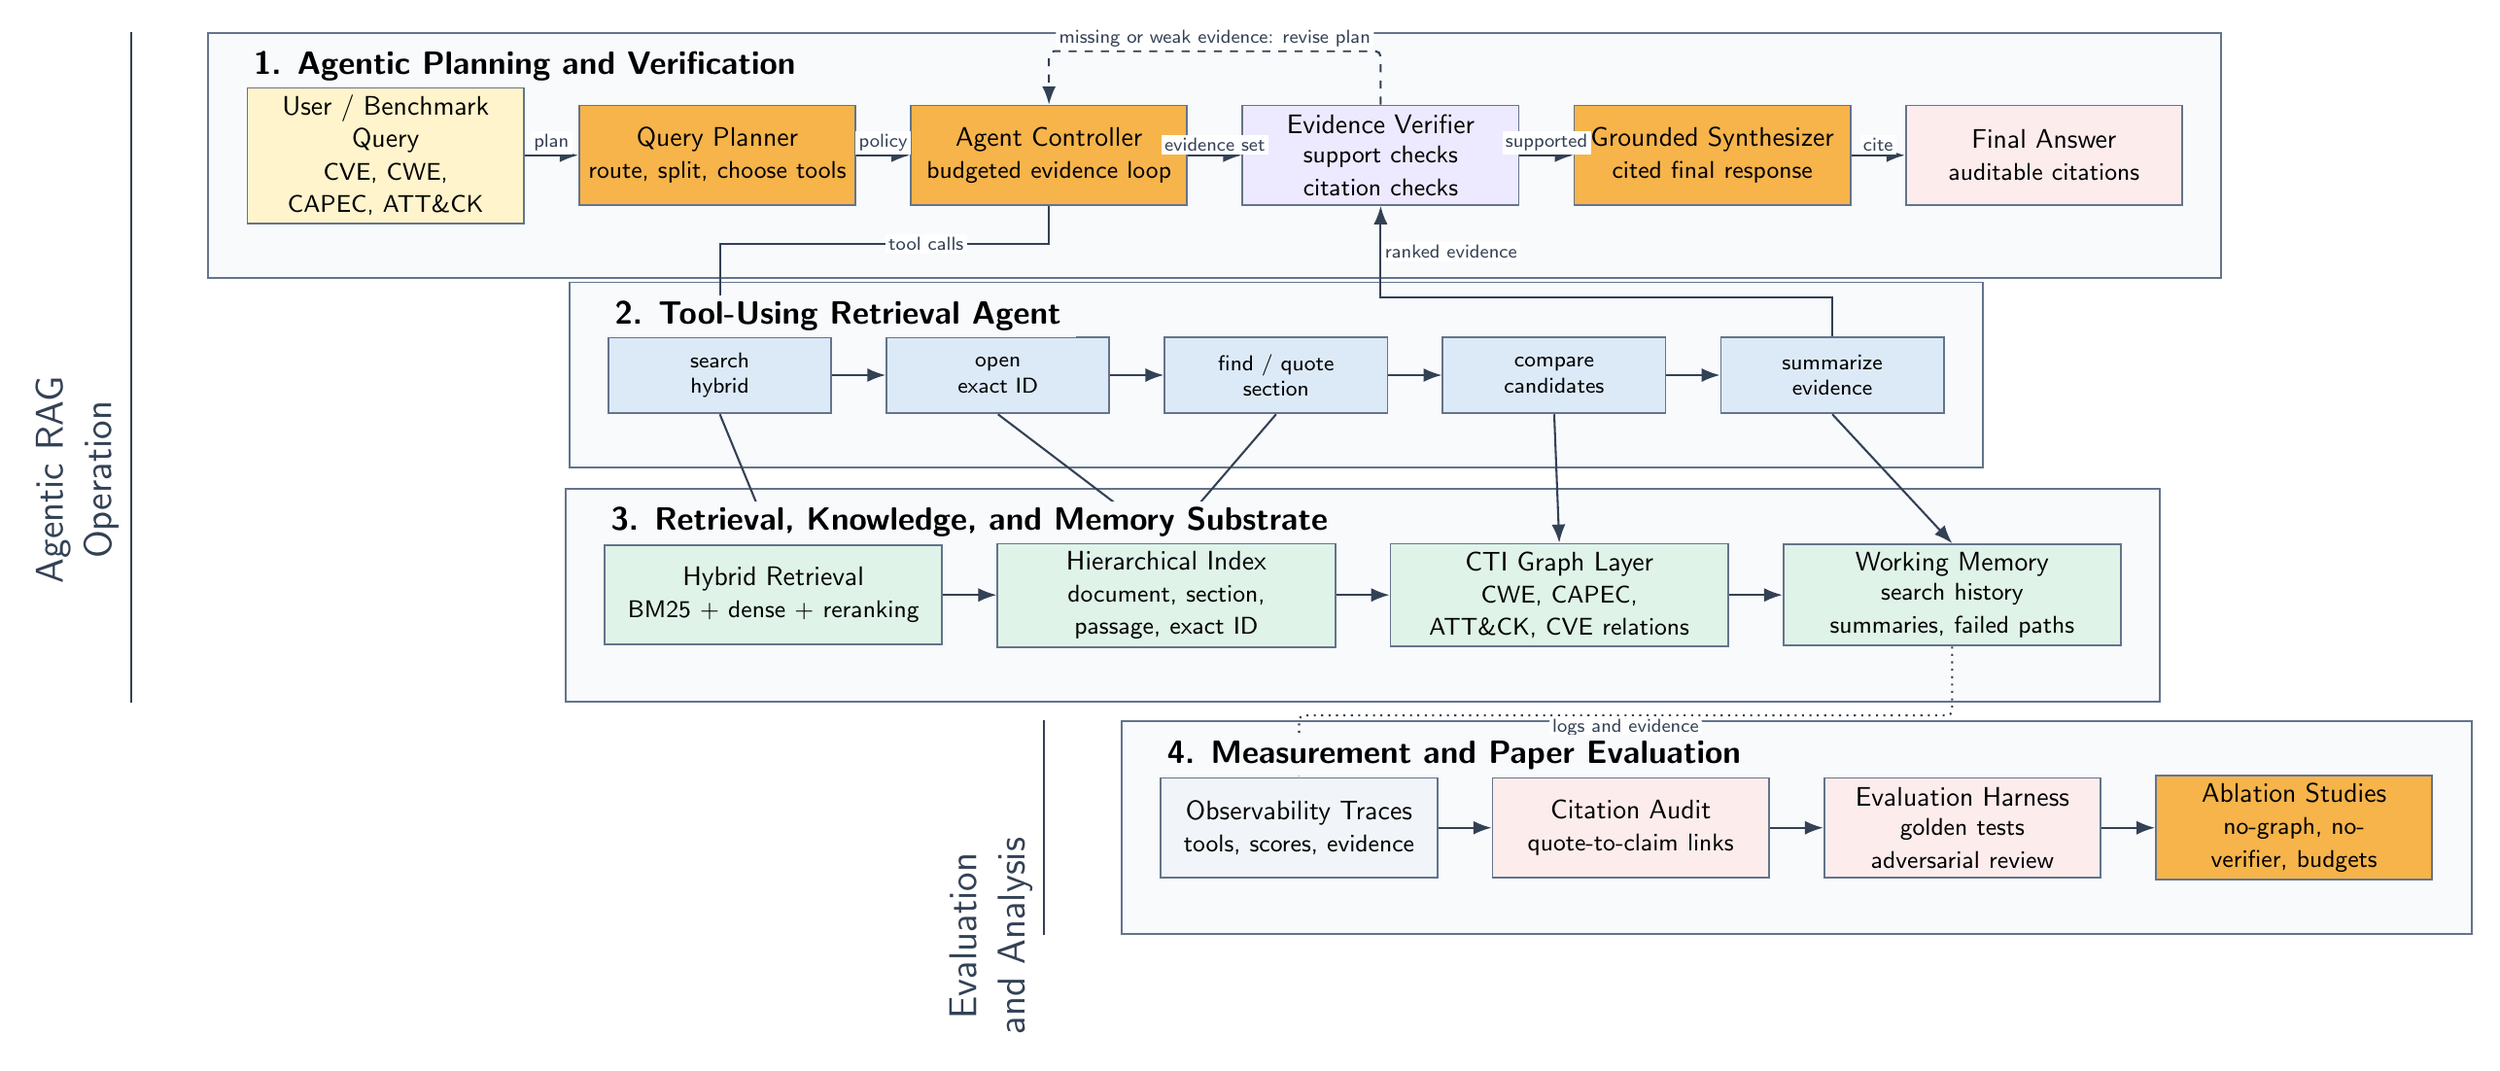
\begin{tikzpicture}[node distance=7mm and 7mm]

% ---------------------------------------------------------------------------
% Main agent workflow
% ---------------------------------------------------------------------------
\node[query] (query) at (0,0)
  {User / Benchmark\\Query\\{\small CVE, CWE, CAPEC, ATT\&CK}};
\node[agent, right=of query] (planner)
  {Query Planner\\{\small route, split, choose tools}};
\node[agent, right=of planner] (controller)
  {Agent Controller\\{\small budgeted evidence loop}};
\node[verifier, right=of controller] (verifier)
  {Evidence Verifier\\{\small support checks\\citation checks}};
\node[agent, right=of verifier] (synth)
  {Grounded Synthesizer\\{\small cited final response}};
\node[eval, right=of synth] (answer)
  {Final Answer\\{\small auditable citations}};

\begin{pgfonlayer}{background}
\node[layer, fit=(query)(planner)(controller)(verifier)(synth)(answer)] (agentlayer) {};
\end{pgfonlayer}

\draw[arrow] (query) -- node[flowlabel, above] {plan} (planner);
\draw[arrow] (planner) -- node[flowlabel, above] {policy} (controller);
\draw[arrow] (controller) -- node[flowlabel, above] {evidence set} (verifier);
\draw[arrow] (verifier) -- node[flowlabel, above] {supported} (synth);
\draw[arrow] (synth) -- node[flowlabel, above] {cite} (answer);

% ---------------------------------------------------------------------------
% Tool layer
% ---------------------------------------------------------------------------
\node[tool, below=17mm of controller, xshift=-43mm] (search)
  {search\\hybrid};
\node[tool, right=of search] (open)
  {open\\exact ID};
\node[tool, right=of open] (quote)
  {find / quote\\section};
\node[tool, right=of quote] (compare)
  {compare\\candidates};
\node[tool, right=of compare] (summarize)
  {summarize\\evidence};

\begin{pgfonlayer}{background}
\node[layer, fit=(search)(open)(quote)(compare)(summarize)] (toollayer) {};
\end{pgfonlayer}

\draw[arrow] (search) -- (open);
\draw[arrow] (open) -- (quote);
\draw[arrow] (quote) -- (compare);
\draw[arrow] (compare) -- (summarize);
\draw[arrow] (controller.south) -- ++(0,-5mm)
  -| node[flowlabel, near start, right] {tool calls} (search.north);
\draw[arrow] (summarize.north) -- ++(0,5mm)
  -| node[flowlabel, near end, right] {ranked evidence} (verifier.south);

% ---------------------------------------------------------------------------
% Knowledge substrate
% ---------------------------------------------------------------------------
\node[knowledge, below=17mm of search, xshift=7mm] (hybrid)
  {Hybrid Retrieval\\{\small BM25 + dense + reranking}};
\node[knowledge, right=of hybrid] (hierarchy)
  {Hierarchical Index\\{\small document, section, passage, exact ID}};
\node[knowledge, right=of hierarchy] (graph)
  {CTI Graph Layer\\{\small CWE, CAPEC, ATT\&CK, CVE relations}};
\node[knowledge, right=of graph] (memory)
  {Working Memory\\{\small search history\\summaries, failed paths}};

\begin{pgfonlayer}{background}
\node[layer, fit=(hybrid)(hierarchy)(graph)(memory)] (knowledgelayer) {};
\end{pgfonlayer}

\draw[arrow] (hybrid) -- (hierarchy);
\draw[arrow] (hierarchy) -- (graph);
\draw[arrow] (graph) -- (memory);
\draw[arrow] (search.south) -- (hybrid.north);
\draw[arrow] (open.south) -- (hierarchy.north);
\draw[arrow] (quote.south) -- (hierarchy.north);
\draw[arrow] (compare.south) -- (graph.north);
\draw[arrow] (summarize.south) -- (memory.north);

% Explicit repair loop.
\draw[feedback] (verifier.north) -- ++(0,7mm)
  -| node[flowlabel, pos=0.25, above] {missing or weak evidence: revise plan} (controller.north);

% ---------------------------------------------------------------------------
% Measurement sidecar
% ---------------------------------------------------------------------------
\node[trace, below=17mm of graph, xshift=-34mm] (trace)
  {Observability Traces\\{\small tools, scores, evidence}};
\node[eval, right=of trace] (audit)
  {Citation Audit\\{\small quote-to-claim links}};
\node[eval, right=of audit] (evalh)
  {Evaluation Harness\\{\small golden tests\\adversarial review}};
\node[agent, right=of evalh] (ablation)
  {Ablation Studies\\{\small no-graph, no-verifier, budgets}};

\begin{pgfonlayer}{background}
\node[layer, fit=(trace)(audit)(evalh)(ablation)] (measurementlayer) {};
\end{pgfonlayer}

\draw[observe] (memory.south) -- ++(0,-9mm)
  -| node[flowlabel, pos=0.25, below] {logs and evidence} (trace.north);
\draw[arrow] (trace) -- (audit);
\draw[arrow] (audit) -- (evalh);
\draw[arrow] (evalh) -- (ablation);

% Side grouping labels.
\coordinate (opTop) at ($(agentlayer.north west)+(-10mm,0)$);
\coordinate (opBottom) at (opTop |- knowledgelayer.south west);
\draw[side rule] (opTop) -- (opBottom)
  node[midway, left=7mm, side label] {Agentic RAG\\Operation};

\coordinate (evalTop) at ($(measurementlayer.north west)+(-10mm,0)$);
\coordinate (evalBottom) at (evalTop |- measurementlayer.south west);
\draw[side rule] (evalTop) -- (evalBottom)
  node[midway, left=7mm, side label] {Evaluation\\and Analysis};

% Draw layer titles last so routing never obscures the text.
\node[layer title, anchor=north west] at ($(agentlayer.north west)+(4mm,-1.8mm)$)
  {1. Agentic Planning and Verification};
\node[layer title, anchor=north west] at ($(toollayer.north west)+(4mm,-1.8mm)$)
  {2. Tool-Using Retrieval Agent};
\node[layer title, anchor=north west] at ($(knowledgelayer.north west)+(4mm,-1.8mm)$)
  {3. Retrieval, Knowledge, and Memory Substrate};
\node[layer title, anchor=north west] at ($(measurementlayer.north west)+(4mm,-1.8mm)$)
  {4. Measurement and Paper Evaluation};

\end{tikzpicture}
\end{document}
